\documentclass[a4paper]{article}
\usepackage{geometry}
\usepackage{graphicx}
\usepackage{natbib}
\usepackage{amsmath}
\usepackage{amssymb}
\usepackage{amsthm}
\usepackage{paralist}
\usepackage{epstopdf}
\usepackage{tabularx}
\usepackage{longtable}
\usepackage{multirow}
\usepackage{multicol}
\usepackage[hidelinks]{hyperref}
\usepackage{fancyvrb}
\usepackage{float}
\usepackage{paralist}
\usepackage[svgname]{xcolor}
\usepackage{enumerate}
\usepackage{array}
\usepackage{times}
\usepackage{url}
\usepackage{fancyhdr}
\usepackage{comment}
\usepackage{environ}
\usepackage{times}
\usepackage{textcomp}
\usepackage{caption}
\usepackage{bbm}
\usepackage{enumitem}
\usepackage{algorithm}
\usepackage{algpseudocode}
\usepackage{caption}
\usepackage{subcaption}


\urlstyle{rm}

\setlength\parindent{0pt} % Removes all indentation from paragraphs
\theoremstyle{definition}
\newtheorem{definition}{Definition}[]
\newtheorem{conjecture}{Conjecture}[]
\newtheorem{example}{Example}[]
\newtheorem{theorem}{Theorem}[]
\newtheorem{lemma}{Lemma}
\newtheorem{proposition}{Proposition}
\newtheorem{corollary}{Corollary}

\floatname{algorithm}{Procedure}
\renewcommand{\algorithmicrequire}{\textbf{Input:}}
\renewcommand{\algorithmicensure}{\textbf{Output:}}
\newcommand{\abs}[1]{\lvert#1\rvert}
\newcommand{\norm}[1]{\lVert#1\rVert}
\newcommand{\RR}{\mathbb{R}}
\newcommand{\CC}{\mathbb{C}}
\newcommand{\Nat}{\mathbb{N}}
\newcommand{\br}[1]{\{#1\}}
\DeclareMathOperator*{\argmin}{arg\,min}
\DeclareMathOperator*{\argmax}{arg\,max}
\renewcommand{\qedsymbol}{$\blacksquare$}

\definecolor{dkgreen}{rgb}{0,0.6,0}
\definecolor{gray}{rgb}{0.5,0.5,0.5}
\definecolor{mauve}{rgb}{0.58,0,0.82}

\newcommand{\Var}{\mathrm{Var}}
\newcommand{\Cov}{\mathrm{Cov}}

\newcommand{\vc}[1]{\boldsymbol{#1}}
\newcommand{\xv}{\vc{x}}
\newcommand{\Sigmav}{\vc{\Sigma}}
\newcommand{\alphav}{\vc{\alpha}}
\newcommand{\muv}{\vc{\mu}}

\newcommand{\red}[1]{\textcolor{red}{#1}}

\def\x{\mathbf x}
\def\y{\mathbf y}
\def\w{\mathbf w}
\def\v{\mathbf v}
\def\E{\mathbb E}
\def\V{\mathbb V}
\def\ind{\mathbbm 1}

% TO SHOW SOLUTIONS, include following (else comment out):
\newenvironment{soln}{
	\leavevmode\color{blue}\ignorespaces
}{}

\hypersetup{
	%    colorlinks,
	linkcolor={red!50!black},
	citecolor={blue!50!black},
	urlcolor={blue!80!black}
}

\geometry{
	top=1in,            % <-- you want to adjust this
	inner=1in,
	outer=1in,
	bottom=1in,
	headheight=3em,       % <-- and this
	headsep=2em,          % <-- and this
	footskip=3em,
}


\pagestyle{fancyplain}
\lhead{\fancyplain{}{Homework 6}}
\rhead{\fancyplain{}{CS 760 Machine Learning}}
\cfoot{\thepage}

\title{\textsc{Homework 6}} % Title

%%% NOTE:  Replace 'NAME HERE' etc., and delete any "\red{}" wrappers (so it won't show up as red)

\author{
	\red{$>>$Martin Diges$<<$} \\
	\red{$>>$9080689699$<<$}\\
} 

\date{}

\begin{document}
	
	\maketitle 
	
        \textbf{Instructions:}
        Use this latex file as a template to develop your homework. Submit your homework on time as a single pdf file. Please wrap your code and upload to a public GitHub repo, then attach the link below the instructions so that we can access it. Answers to the questions that are not within the pdf are not accepted. This includes external links or answers attached to the code implementation. Late submissions may not be accepted. You can choose any programming language (i.e. python, R, or MATLAB). Please check Piazza for updates about the homework. It is ok to share the results of the experiments and compare them with each other.
        \vspace{0.1in}

        \\\\
        \hypersetup{colorlinks=true, linkcolor=cyan}
        \url{https://github.com/missingnoglitch0/cs760/tree/main/hw6}
	
	\section{Implementation: GAN (50 pts)}
	In this part, you are expected to implement GAN with MNIST dataset. We have provided a base jupyter notebook (gan-base.ipynb) for you to start with, which provides a model setup and training configurations to train GAN with MNIST dataset.
	
	\begin{enumerate} [label=(\alph*)]

            %%% 1.1
            
		\item Implement training loop and report learning curves and generated images in epoch 1, 50, 100. Note that drawing learning curves and visualization of images are already implemented in provided jupyter notebook. \hfill (20 pts)
		
		\begin{algorithm}
			\caption{Training GAN, modified from \cite{goodfellow2014generative}}\label{alg:GAN}
			\begin{algorithmic}
				% \Require $m$: real data batch size, $n_{z}$: fake data batch size
				\Ensure Discriminator $D$, Generator $G$
				
				\For{number of training iterations}
				
				\State{$\#$ Training discriminator}
				\State{Sample minibatch of $m$ noise samples $\{z^{(1)}, z^{(2)}, \cdots, z^{(m)}\}$ from noise prior $p_{g}(z)$}
				\State{Sample minibatch of $m$ examples $\{x^{(1)}, x^{(2)}, \cdots, x^{(m)}\}$} from the data
				\State{Update the discriminator by ascending its stochastic  gradient:
					$$\nabla_{\theta_{d}} \big ( \cfrac{1}{m}  \sum_{i=1}^{m}  \log D(x^{(i)})  + \cfrac{1}{m} \sum_{i=1}^{m}  \log (1-D(G(z^{(i)})))\big )$$
				}
				
				\State{$\#$ Training generator}
				\State{Sample minibatch of $m$ noise samples $\{z^{(1)}, z^{(2)}, \cdots, z^{(m)}\}$ from noise prior $p_{g}(z)$}
				\State{Update the generator  by ascending its stochastic  gradient:
					$$\nabla_{\theta_{g}}  \cfrac{1}{m} \sum_{i=1}^{m}  \log D(G(z^{(i)}))\big )$$
				}
				\EndFor
				
				\State{$\#$ The gradient-based updates can use any standard gradient-based learning rule. In the base code, we are using Adam optimizer \citep{kingma2014adam}}
			\end{algorithmic}
		\end{algorithm}

            %%% Solution
		\begin{soln}
                \begin{figure}[H]
    			\centering
    			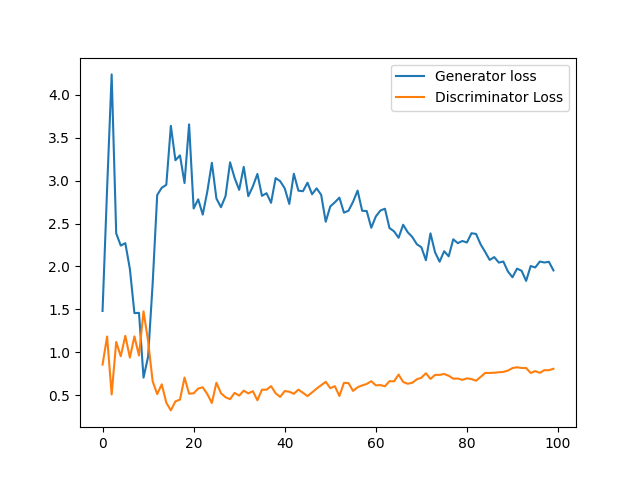
\includegraphics[width=0.7\textwidth]{hw6/1.a/1_a_loss.png}
    			\caption{Learning curve}
    			\label{fig:gan_q1_loss}
    		\end{figure}
    		
    		\begin{figure}[H]
    			\centering
    			\begin{subfigure}[b]{0.3\textwidth}
    				\centering
    				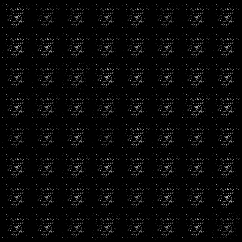
\includegraphics[width=\textwidth]{hw6/1.a/1_a_gen_img1.png}
    				\caption{epoch 1}
    			\end{subfigure}
    			\hfill
    			\begin{subfigure}[b]{0.3\textwidth}
    				\centering
    				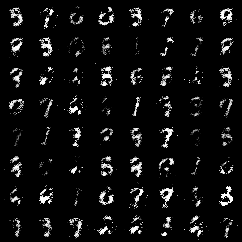
\includegraphics[width=\textwidth]{hw6/1.a/1_a_gen_img50.png}
    				\caption{epoch 50}
    			\end{subfigure}
    			\hfill
    			\begin{subfigure}[b]{0.3\textwidth}
    				\centering
    				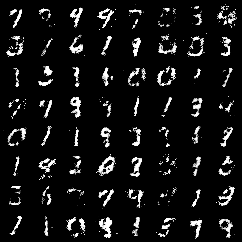
\includegraphics[width=\textwidth]{hw6/1.a/1_a_gen_img100.png}
    				\caption{epoch 100}
    			\end{subfigure}
    			\caption{Generated images by $G$}
    			\label{fig:three graphs}
    		\end{figure}
            \end{soln}
		

            %%% 1.2
  
		\newpage
		\item Replace the generator update rule as the original one in the slide,\\
		``Update the generator by descending its stochastic gradient:
		
		$$\nabla_{\theta_{g}}  \cfrac{1}{n_{z}}  \sum_{i=1}^{n_{z}}\log (1-D(G(z^{(i)})))\big )$$
		"
		, and report learning curves and generated images in epoch 1, 50, 100. Compare the result with (a). Note that it may not work. If training does not work, explain why it doesn't work. \\
        You may find this helpful: https://jonathan-hui.medium.com/gan-what-is-wrong-with-the-gan-cost-function-6f594162ce01
		\hfill (10 pts)
		
		\begin{soln}
                \begin{figure}[H]
    			\centering
    			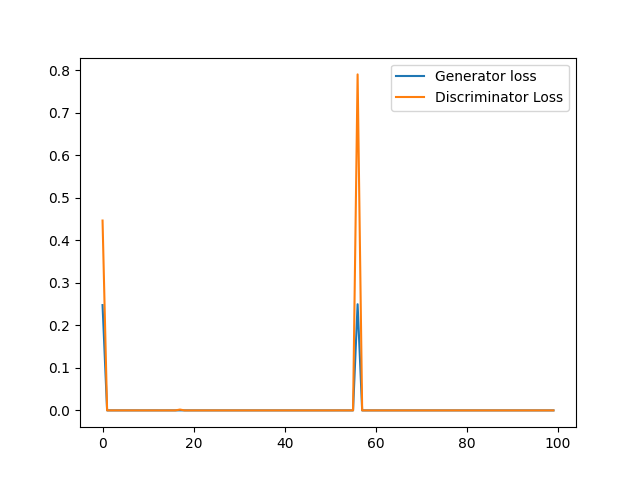
\includegraphics[width=0.7\textwidth]{hw6/1.b/1_b_loss.png}
    			\caption{Learning curve}
    			\label{fig:gan_q1_loss}
    		\end{figure}
    		
    		\begin{figure}[H]
    			\centering
    			\begin{subfigure}[b]{0.3\textwidth}
    				\centering
    				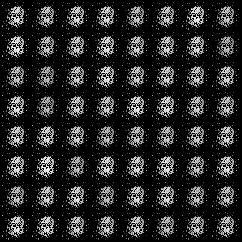
\includegraphics[width=\textwidth]{hw6/1.b/1_b_gen_img1.png}
    				\caption{epoch 1}
    			\end{subfigure}
    			\hfill
    			\begin{subfigure}[b]{0.3\textwidth}
    				\centering
    				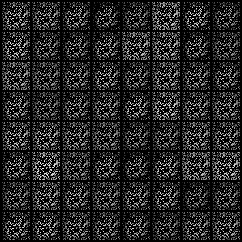
\includegraphics[width=\textwidth]{hw6/1.b/1_b_gen_img50.png}
    				\caption{epoch 50}
    			\end{subfigure}
    			\hfill
    			\begin{subfigure}[b]{0.3\textwidth}
    				\centering
    				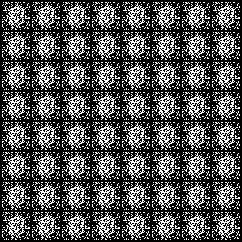
\includegraphics[width=\textwidth]{hw6/1.b/1_b_gen_img100.png}
    				\caption{epoch 100}
    			\end{subfigure}
    			\caption{Generated images by $G$}
    			\label{fig:three graphs}
    		\end{figure}

            Compared with (a), the generator in (b) does not produce images which are recognisable as close to those of the source distribution. In short, the training did not work. The training did not work because the gradient provided quickly vanishes to near-0 values. From Jonathan Hui's post, Corollary 2.1 tells us that the gradient above vanishes when the discriminator becomes optimal. Thus, the generator does not significantly change and the discriminator, which is already doing a sufficiently good job w.r.t to its gradient, also stops meaningfully changing.
            \end{soln}

            %%% 1.3
            \newpage
		\item Except the method that we used in (a), how can we improve training for GAN? Implement that and report your setup, learning curves, and generated images in epoch 1, 50, 100.
        This question is an open-ended question and you can choose whichever method you want.
		\hfill (20 pts)
		
		\begin{soln}  
  
                \begin{figure}[H]
    			\centering
    			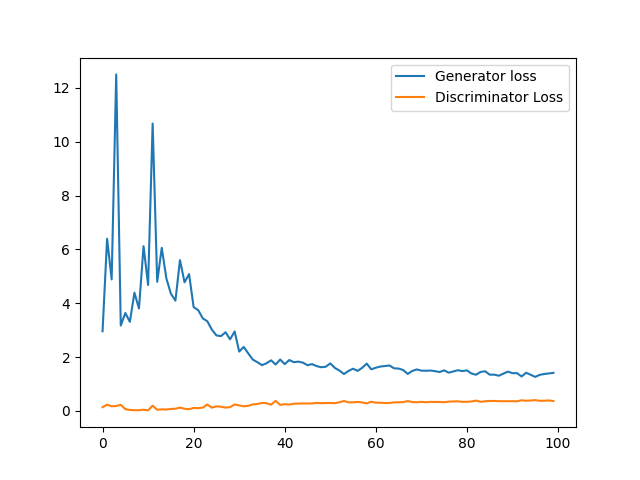
\includegraphics[width=0.7\textwidth]{hw6/1.c/1_c_loss.png}
    			\caption{Learning curve}
    			\label{fig:gan_q1_loss}
    		\end{figure}
    		
    		\begin{figure}[H]
    			\centering
    			\begin{subfigure}[b]{0.3\textwidth}
    				\centering
    				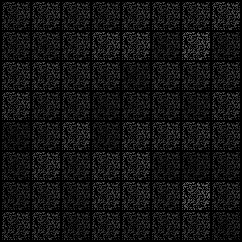
\includegraphics[width=\textwidth]{hw6/1.c/1_c_gen_img1.png}
    				\caption{epoch 1}
    			\end{subfigure}
    			\hfill
    			\begin{subfigure}[b]{0.3\textwidth}
    				\centering
    				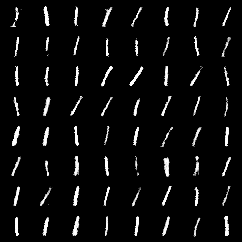
\includegraphics[width=\textwidth]{hw6/1.c/1_c_gen_img100.png}
    				\caption{epoch 50}
    			\end{subfigure}
    			\hfill
    			\begin{subfigure}[b]{0.3\textwidth}
    				\centering
    				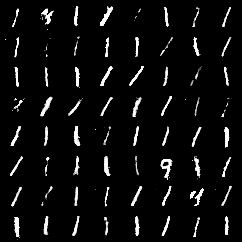
\includegraphics[width=\textwidth]{hw6/1.c/1_c_gen_img200.png}
    				\caption{epoch 100}
    			\end{subfigure}
    			\caption{Generated images by $G$}
    			\label{fig:three graphs}
    		\end{figure}

                One way to improve training for GAN is to use a k:1 ratio of discriminator update steps to generator update steps. This is described in the original paper on GAN by Goodfellow et al. We do k steps of discriminator training for every 1 step of generator training. For this model in particular, we set k=2.
                Internally, this is implemented by multiplying the original number of epochs by k and only running the generator update step when bi \% k = k-1; i.e. after every k discriminator updates, the generator updates once.
                
                This of course increases training time (For my implementation, roughly double). However, for the same number of generator update steps, the generator in (c) has consistently lower error. After 50 generator update steps, the generator in (a) has error around 2.5, whereas the generator in (c) has error around 1.6. After 100 generator update steps, the generator in (a) has error around 2.0, whereas the generator in (c) has error around 1.35.
                One interesting observation is that the generator in (c) experiences mode collapse (the model tends to generate digits that resemble the number 1, as these seem to be the easiest to get past the discriminator). In this sense, the model is a failure. But, from the perspective of making realistic digits, the model is a success. It achieves consistently lower generator loss than (a).
      
            \end{soln}
		
	\end{enumerate}

\newpage

\section{Directed Graphical Model [25 points]}
Consider the directed graphical model (aka Bayesian network) in Figure~\ref{fig:bn}.
\begin{figure}[H]
    \centering
    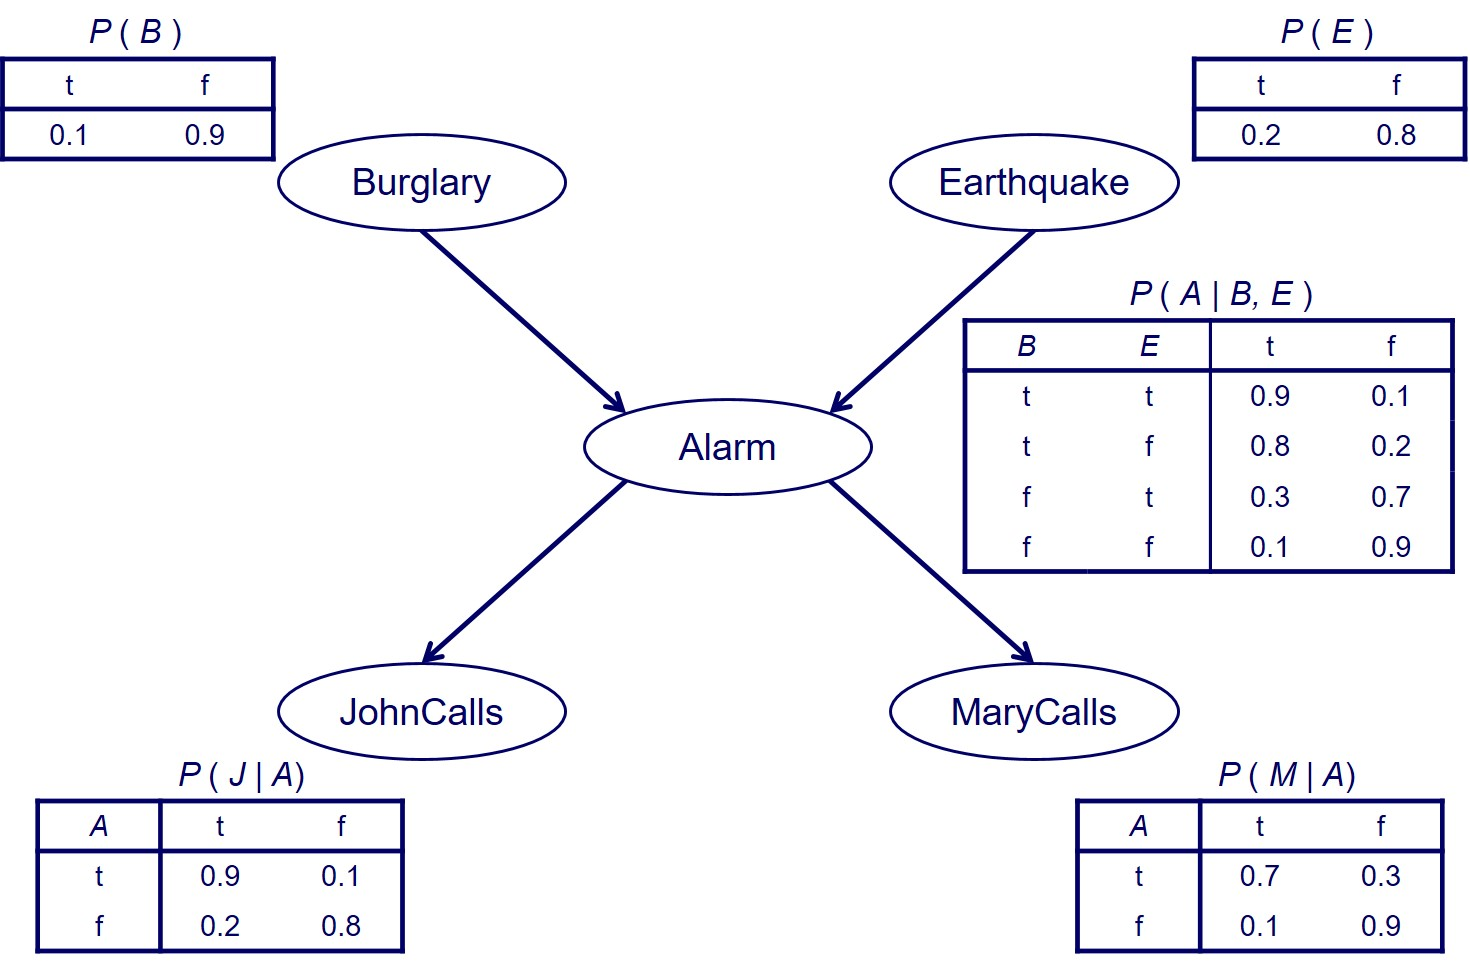
\includegraphics[width=0.8\textwidth]{BN.jpeg}
    \caption{A Bayesian Network example.}
    \label{fig:bn}
\end{figure}
Compute $P(B=t \mid E=f,J=t,M=t)$ and $P(B=t \mid E=t,J=t,M=t)$. (10 points for each) These are the conditional probabilities of a burglar in your house (yikes!) when both of your neighbors John and Mary call you and say they hear an alarm in your house, but without or with an earthquake also going on in that area (what a busy day), respectively.

\begin{soln}
We define $v \implies V = t$ and $\neg v \implies V = f$ for a variable $V$. \\
Additionally, we establish that
$$P(B, E, j, m) = \sum_{a, \neg a} P(B) P(E) P(A | B, E) P(j | A) P(m | A) = P(B) P(E) \sum_{a, \neg a} P(A | B, E) P(j | A) P(m | A)$$

\begin{itemize}
    \item $P(B=t \mid E=f,J=t,M=t) = P(b | \neg e, j, m) =
    \frac{P(b, \neg e, j, m)}{P(\neg e, j, m)} = \frac{P(b, \neg e, j, m)}{P(b, \neg e, j, m) + P(\neg b, \neg e, j, m)}$

    \begin{itemize}
        \item $P(b, \neg e, j, m) = P(b) P(\neg e) \sum_{a, \neg a} P(A | b, \neg e) P(j | A) P(m | A)$ \\
        $= (0.1 * 0.8)([0.8 * 0.9 * 0.7] + [0.2 * 0.2 * 0.1]) = 0.04064$

        \item $P(\neg b, \neg e, j, m) = P(\neg b) P(\neg e) \sum_{a, \neg a} P(A | \neg b, \neg e) P(j | A) P(m | A)$ \\
        $= (0.9 * 0.8)([0.1 * 0.9 * 0.7] + [0.9 * 0.2 * 0.1]) = 0.05832$
    \end{itemize}

    \textbf{Finally, we have that}
 
    $P(B=t \mid E=f,J=t,M=t) = \frac{0.04064}{0.04064 + 0.05832} = 0.4106$
    
    \item $P(B=t \mid E=t,J=t,M=t) = P(b | e, j, m) =
    \frac{P(b, e, j, m)}{P(e, j, m)} = \frac{P(b, e, j, m)}{P(b, e, j, m) + P(\neg b, e, j, m)}$

    \begin{itemize}
        \item $P(b, e, j, m) = P(b) P(e) \sum_{a, \neg a} P(A | b, e) P(j | A) P(m | A)$ \\
        $= (0.1 * 0.2)([0.9 * 0.9 * 0.7] + [0.1 * 0.2 * 0.1]) = 0.01138$

        \item $P(\neg b, e, j, m) = P(\neg b) P(e) \sum_{a, \neg a} P(A | \neg b, e) P(j | A) P(m | A)$ \\
        $= (0.9 * 0.2)([0.3 * 0.9 * 0.7] + [0.7 * 0.2 * 0.1]) = 0.03654$
    \end{itemize}

    \textbf{Finally, we have that}

    $P(B=t \mid E=t,J=t,M=t) = \frac{0.01138}{0.01138 + 0.03654} = 0.2375$
    
\end{itemize}

\end{soln}

\newpage

\section{Chow-Liu Algorithm [25 pts]}
Suppose we wish to construct a directed graphical model for 3 features $X$, $Y$, and $Z$ using the Chow-Liu algorithm. We are given data from 100 independent experiments where each feature is binary and takes value $T$ or $F$. Below is a table summarizing the observations of the experiment:

\begin{table}[H]
        \centering
                \begin{tabular}{cccc}
                           $X$ & $Y$ & $Z$ & Count \\
                                \hline
                                T & T & T & 36 \\
                                \hline
                                T & T & F & 4 \\
                                \hline
                                T & F & T & 2 \\
                                \hline
                                T & F & F & 8 \\
                                \hline
                                F & T & T & 9 \\
                                \hline
                                F & T & F & 1 \\
                                \hline
                                F & F & T & 8 \\
                                \hline
                                F & F & F & 32 \\
                                \hline
                \end{tabular}
\end{table}

\begin{enumerate}
	\item Compute the mutual information $I(X, Y)$ based on the frequencies observed in the data. (5 pts)

        Please see \text{chow\_liu.ipynb} in the GitHub repo for code which calculates mutual informations.

        To proceed with questions 3.1-3.3, we calculate the following:

        P(X) = {True: 0.5, False: 0.5}\\
        P(Y) = {True: 0.5, False: 0.5}\\
        P(Z) = {True: 0.55, False: 0.45}\\
        P(X, Y) = {(True, True): 0.4, (True, False): 0.1, (False, True): 0.1, (False, False): 0.4}\\
        P(X, Z) = {(True, True): 0.38, (True, False): 0.12, (False, True): 0.17, (False, False): 0.33}\\
        P(Z, Y) = {(True, True): 0.45, (True, False): 0.1, (False, True): 0.05, (False, False): 0.4}\\

        And we restate the mutual information formula:

        $$I(X,Y) = \sum_{v \in values(X)} \sum_{y \in values(Y)} P(x,y) \log_2{\frac{P(x,y)}{P(x)P(y)}}$$

        \textbf{ANSWER}\\
        I(X, Y) = 0.27807190511263774 = \\
        0.4 * log2(0.4/(0.5 * 0.5))= 0.4 * log2(1.6)= 0.2712287620450551\\
        +0.1 * log2(0.1/(0.5 * 0.5))= 0.1 * log2(0.4)= -0.1321928094887362\\
        +0.1 * log2(0.1/(0.5 * 0.5))= 0.1 * log2(0.4)= -0.1321928094887362\\
        +0.4 * log2(0.4/(0.5 * 0.5))= 0.4 * log2(1.6)= 0.2712287620450551\\
 
	\item Compute the mutual information $I(X, Z)$ based on the frequencies observed in the data. (5 pts)

        \textbf{ANSWER}\\
        I(X, Z) = 0.1328449618090321 = \\
        0.38 * log2(0.38/(0.5 * 0.55))= 0.38 * log2(1.3818181818181816)= 0.17729576396919175\\
        +0.12 * log2(0.12/(0.5 * 0.45))= 0.12 * log2(0.5333333333333333)= -0.10882687147302222\\
        +0.17 * log2(0.17/(0.5 * 0.55))= 0.17 * log2(0.6181818181818182)= -0.11796246828663445\\
        +0.33 * log2(0.33/(0.5 * 0.45))= 0.33 * log2(1.4666666666666668)= 0.18233853759949703\\
 
	\item Compute the mutual information $I(Z, Y)$ based on the frequencies observed in the data. (5 pts)

        \textbf{ANSWER} \\
        I(Z, Y) = 0.39731260974948646 = \\
        0.45 * log2(0.45/(0.55 * 0.5))= 0.45 * log2(1.6363636363636362)= 0.3197220222622567\\
        +0.1 * log2(0.1/(0.55 * 0.5))= 0.1 * log2(0.36363636363636365)= -0.14594316186372974\\
        +0.05 * log2(0.05/(0.45 * 0.5))= 0.05 * log2(0.22222222222222224)= -0.10849625007211561\\
        +0.4 * log2(0.4/(0.45 * 0.5))= 0.4 * log2(1.777777777777778)= 0.3320299994230751\\

        \newpage
 
	\item Which undirected edges will be selected by the Chow-Liu algorithm as the maximum spanning tree? (5 pts)

        \textbf{ANSWER}
        
        We can use Kruskal's algorithm to obtain an MST: 
        
        We sort the edges in descending weight to get:
        \begin{itemize}
            \item I(Z, Y)
            \item I(X, Y)
            \item I(X, Z)
        \end{itemize}

        Then, we take every edge  which does not cause a cycle, starting with the first.
        (Z,Y) and (X,Y) can be picked without causing a cycle.
        
	\item Root your tree at node $X$, assign directions to the selected edges. (5 pts)

        \textbf{ANSWER}
        
        $X \longrightarrow Y$ and $Y \longrightarrow Z$.
        
\end{enumerate}

	\bibliography{hw6}
	\bibliographystyle{apalike}
\end{document}
